To a large extent, workload determines the time exposed to failure. With other factors being the same, an application with a larger workload is likely to encounter more failures during its execution. Hence, it is intuitive that workload would impact the performance comparison among the three fault tolerance approaches. 

Fixing $N$ at 1,000,000, we increase $W$ from 1,000,000 hours to 12,000,000 hours. Figure~\ref{fig:w25} assumes a MTBF of 25 years and shows the time and energy in log-scale. Checkpointing has the worst performance in both time and energy in all cases. In terms of completion time, process replication is more effcient than Lazy Shadowing when workload reaches 6,000,000 hours. Considering energy consumption, however, Lazy Shadowing is able to achieve the most energy saving in all cases. When MTBF of 25 years is used, the difference is that process repliaction consumes than energy than Lazy Shadowing when $W$ reaches 6,000,000.

\begin{figure*}[!h]
	\begin{center}
		\subfigure[Expected completion time]
		{
			\label{fig:wt25}
			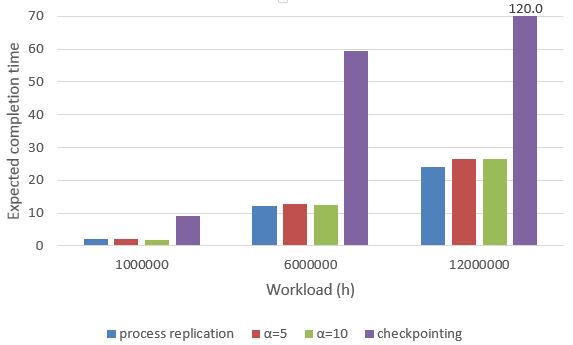
\includegraphics[width=\columnwidth]{Figures/wt25}
		} 
		\subfigure[Expected energy consumption]
		{
			\label{fig:we25}
			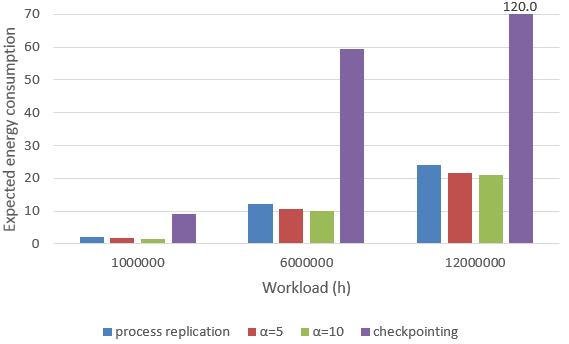
\includegraphics[width=\columnwidth]{Figures/we25}
		} 
	\end{center}
	\caption{Sensitivity to workload. $N=1,000,000$, $MTTI=25$ years, $\rho=0.5$.}
	\label{fig:w25}
\end{figure*}